\chapter{Bitcoin Cash}
\label{cha:bch}

"Imagine you have a dollar in your wallet, and you put it aside for a while and 
then realise that one coin has split in two. Sounds weird? Not in the cryptocurrency 
world." That is an analogy with the fiat currency reported in an article of 
Shouth China Morning Post\cite{scmp}.
Bitcoin is like a software, but, due to its distributed nature, unlike all the 
software we know, there isn't a single entity who determines how it should be 
updated. As a result, to upgrade the blockchain it is necessary to be in 
agreement with the major part of the community. That's what happened on July 20th,
2017, when the 97\% of the Bitcoin network voted to activate the "Segregated 
Witness" (SegWit) algorithm \ref{sec:segwit} to improve the scalability of Bitcoin. Altough almost 
all the comumnity agreed, some members believed that adopting SegWit without 
increasing the block size simply postpone the scalability problem of Bitcoin.
As a result, on August 1st, 2017 there were two forks of the Bitcoin network. 
One for adopting SegWit and one incrementing the size of tha blocks giving 
birth to the Bitcoin Cash blockchain.\cite{scmp}\cite{thecryptonomist}

\section{Fork}
\label{sec:fork}

As said before, to have an upgrade in a blockchain we need the agreement of all
the network, those updates are called "forks". Basically, there are two types 
of fork:
\bigskip\\
\textbf{Soft Fork}
means that change in the blockchain protocol is backward-compatible. That means,
that altough some nodes of the network are outdated, they are still able to 
process transaction on the network, as long as they don't brake the new protocol rules.
That's what happened with SegWit in August 2017.
\bigskip\\
\begin{figure}
    \centering
    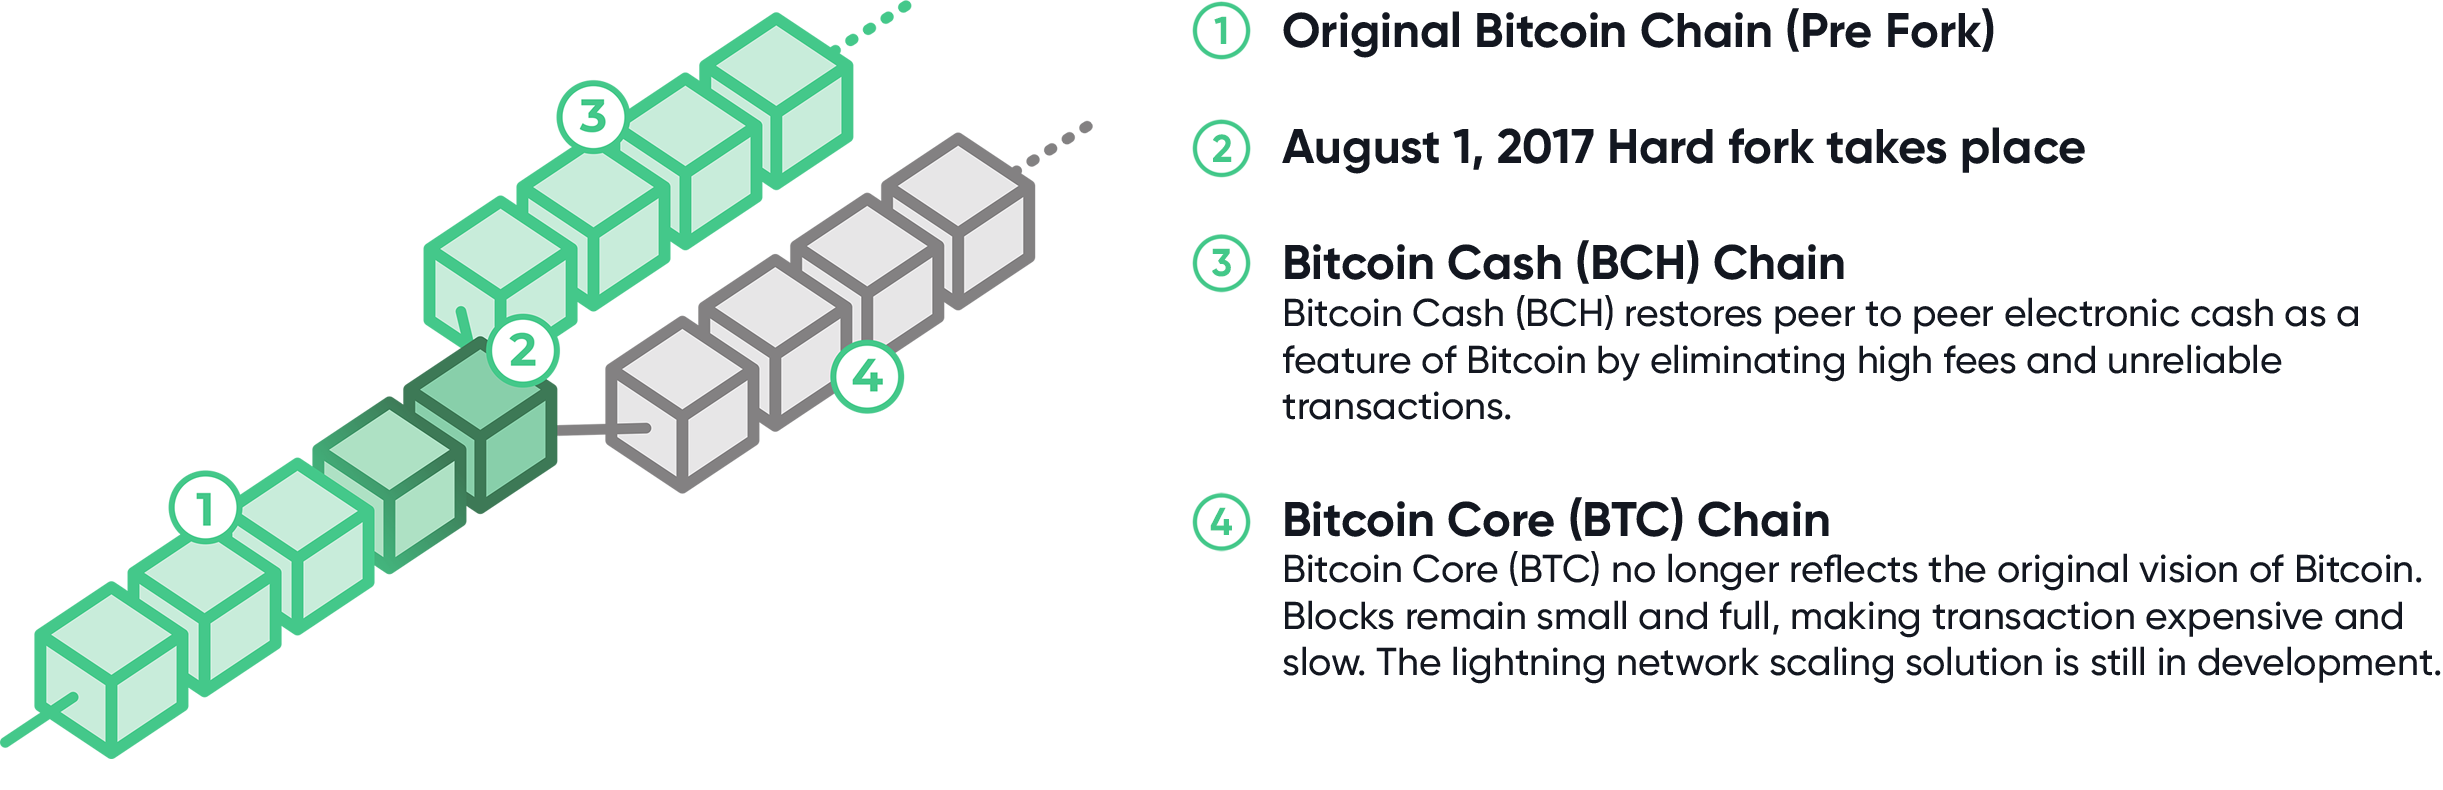
\includegraphics[height=5cm]{fork-img.png}
    \caption{A simple schema of the controversial hark fork of Bitcoin Cash. From \cite{bitcoin.com}}
    \label{fig:hardfork}
\end{figure}
\textbf{Hard Fork}
is the opposite. An obsolete node cannot perform any transaction on the new protocol.
According to the situation, hard fork can either be planned or controversial.
In a planed fork, participants are going to upgrade their software voluntarily,
leaving the old verision behind. The non-update nodes, are going to mine on the old 
blockchain, which will be used by very few participants.\\
In a controversial fork instead, there is a disagreement within the community about
the upgrade, so, the old blockchain is splitted in two new incompatible ones.\\ 
Both will have their own network, and as it happened to Bitcoin Cash on August 2017, 
will be developed in the way the participants believe is the best. Here, is where 
comes to help the analogy made at the beginning, because, all the coins owned before 
the fork, will be splitted. So, the same amout of coins as before will be owned in 
both the blockchains.\cite{binancevision}


\subsection{SegWit}
\label{sec:segwit}

Segregated Witness is the major discrepancy between Bitcoin and Bitcoin Cash. In Fact,
unlike BCH, where to increase the number of transactions per second (TPS)
the block size was only incremented to 8 MegaByte, with SegWit the upgrade was more 
complicated. The transaction is splitted in two segments, the first, which is saved 
on the blockchain, contains the iformation about the sender and the receiver. 
Meanwhile, the second part containing the scripts and the signatrue remain at the 
bottom in a separeate structure. As a result, the amount of information per transaction
its less and makes possible to add more transaction in each block.\\
This is only one of the multiple benefits taken by the adoption of SegWit 
algorithm\footnote{To read about all the benefits of this algortighm read here:
 \url{https://bitcoincore.org/en/2016/01/26/segwit-benefits/}}.

\subsection{Addresses}
\label{sec:addresses}

Due to the nature of Bitcoin Cash, its addresses are generated in exactly the same 
manner as the Bitcoin ones, so it is very difficult to recognize the source of 
a specific address. To facilitate its use and decrease the probability of beeing 
confused when someone tries to read id, was introduced the new Cashaddr Address 
Format. In few words, its only a new type of encoding which will display the 
address with a different pattern. In addition, every new Cashaddr corresponds to 
an old address, so if necessary, also the outdated addresses can be used.

\subsection{Block mining}
\label{sec:mining}

With the fork on August 1st, 2017, Bitcoin Cash not only changes the block size, but 
implements also the "Emergency Difficulty Adjustment" (EDA) algorithm. The motivation was 
to have mean through convince miners to expend thir resources in BCH. In fact, at the 
beginning, even the price of Bitcoin Cash was significantly lower than the price of 
Bitcoin, due to the fork process, the difficulty for mining was the same. So, it was 
less convenience to mine in the BCH blockchain. EDA resolves this problem by reducing 
the difficulty for block number $t$ by 20\% if the time difference between the 
$(t-6)^{th}$ block and $(t-12)^{th}$ block was greater than 12 hours. This system was 
active from 1st August 2017, until 12th November 2017. Indeed, the next day, a hard fork
was made to implement the new "Difficulty Adjustment Algorithm" (DAA), which seeks to 
accomplish the following objectives:
\begin{itemize}
    \item Adjust difficulty to hash rate to target a mean block interval of 600 seconds.
    \item Avoid sudden changes in difficulty when hash rate is fairly stable.
    \item Adjust difficulty rapidly when hash rate changes rapidly.
    \item Avoid oscillations from feedback between hash rate and difficulty.
    \item Be resilient to attacks such as timestamp manipulation.
\end{itemize}
To fulfill all these requirements, the new algorithm adjusts the difficulty with each
block, taking into account the amount of work done and the elapsed time of the previous 
144 blocks.\cite{bitcoinabc}\cite{eda}\pagebreak
